\documentclass[tikz,border=2pt]{standalone}
\usepackage{amsmath,amssymb}
\usepackage{tikz}
\usetikzlibrary{arrows.meta}

\begin{document}
% Conditional pmf from a joint table: keep the column Y = 1 and divide it by its total p_Y(1).
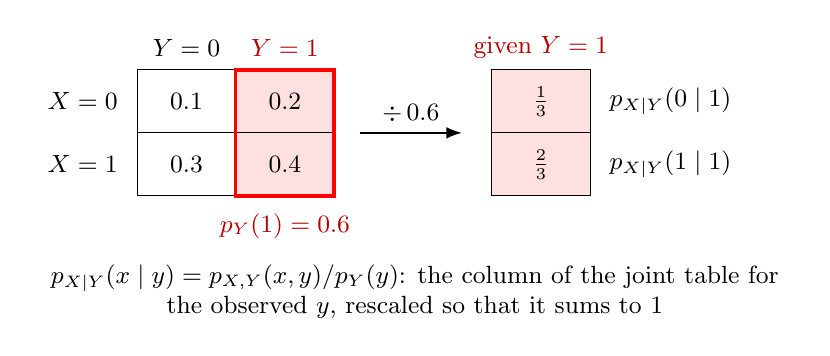
\begin{tikzpicture}[every node/.style={font=\small}, >={Latex[length=2mm]}, cell/.style={draw, minimum width=1.25cm, minimum height=0.8cm}]
	\node[cell] at (0,0) {$0.1$};
	\node[cell, fill=red!12] at (1.25,0) {$0.2$};
	\node[cell] at (0,-0.8) {$0.3$};
	\node[cell, fill=red!12] at (1.25,-0.8) {$0.4$};
	\node[font=\small] at (0,0.68) {$Y=0$};
	\node[font=\small, red!70!black] at (1.25,0.68) {$Y=1$};
	\node[font=\small, anchor=east] at (-0.75,0) {$X=0$};
	\node[font=\small, anchor=east] at (-0.75,-0.8) {$X=1$};
	\draw[red, very thick] (0.625,0.4) rectangle (1.875,-1.2);
	\node[red!70!black, font=\small, anchor=north] at (1.25,-1.3) {$p_Y(1)=0.6$};
	\draw[->, thick] (2.2,-0.4) -- (3.5,-0.4) node[midway, above, font=\small] {$\div\,0.6$};
	\node[cell, fill=red!12] at (4.5,0) {$\tfrac13$};
	\node[cell, fill=red!12] at (4.5,-0.8) {$\tfrac23$};
	\node[font=\small, red!70!black] at (4.5,0.68) {given $Y=1$};
	\node[font=\small, anchor=west] at (5.25,0) {$p_{X\mid Y}(0\mid1)$};
	\node[font=\small, anchor=west] at (5.25,-0.8) {$p_{X\mid Y}(1\mid1)$};
	\node[anchor=north, align=flush center, text width=9.6cm] at (2.9,-1.95) {$p_{X\mid Y}(x\mid y)=p_{X,Y}(x,y)/p_Y(y)$: the column of the joint table for the observed $y$, rescaled so that it sums to $1$};
\end{tikzpicture}
\end{document}
